\documentclass{standalone}
\usepackage{tikz, pgfplots, xcolor}

\definecolor{LB1}{RGB}{17,117,167}
\definecolor{LB2}{RGB}{60,84,111}

\begin{document}
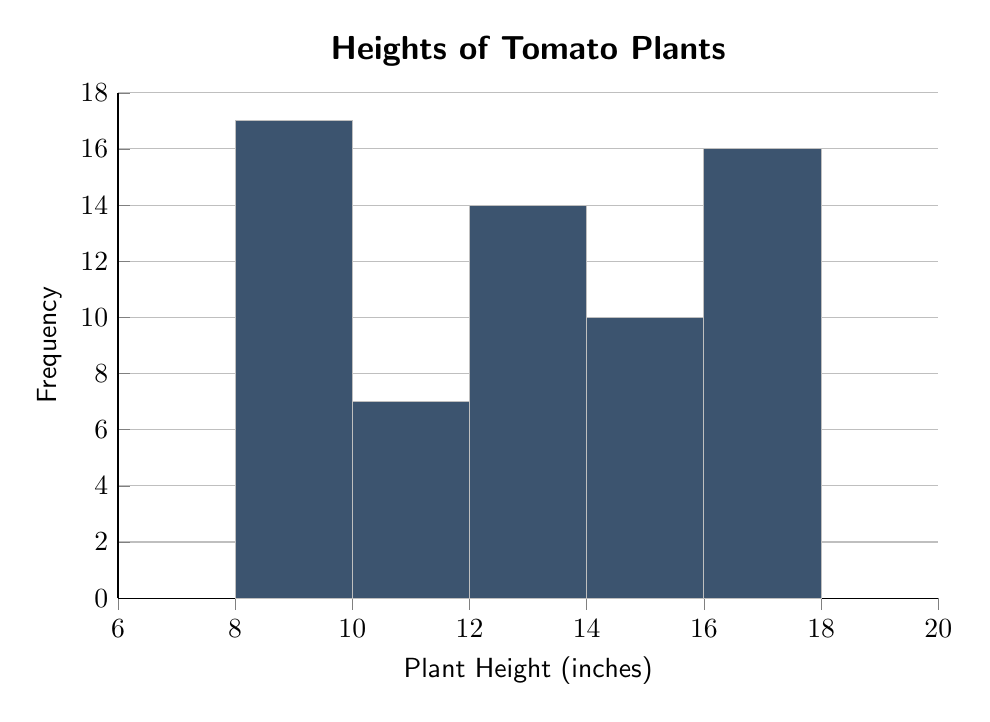
\begin{tikzpicture}
  \begin{axis}[
      axis lines*=left,
      no markers,
      xmin=6, xmax=20, ymin=0, ymax=18,
      ytick={0,2,...,18},
      xlabel style={font=\sffamily},
      xlabel={Plant Height (inches)},
      ylabel style={font=\sffamily},
      ylabel={Frequency},
      title={\large\bfseries\sffamily Heights of Tomato Plants},
      ticklabel style={font=\sffamily},
      enlargelimits=false,
      clip=false,
      grid = none,
      ymajorgrids=true,
      ybar=0pt,
      width=12cm,
      height=8cm
    ]
    \addplot+[ybar interval,fill=LB2, draw=lightgray] plot coordinates { (8, 17) (10, 7) (12, 14) (14, 10) (16, 16) (18,0) };
  \end{axis}
\end{tikzpicture}
\end{document}